
\section{Microcontrolador}

Microcontroladores são circuitos integrados compactos desenvolvidos para governar
uma operação específica em um sistema embarcado. No contexto da aplicação deste
trabalho, o uso de um microcontrolador é fundamental para se obter o controle
desejado de trajetória e posicionamento do robô.

Foram testadas duas placas de microcontrolador o BluePill e ESP32 Devkit v1
Ambas poderiam ser alimentadas através dos pinos de 5v e 3.3v, mas também através do connector micro-USB-B

\subsection{BluePill - STM32F103C8}

A placa BluePill embarca o microcontrolador STM32F103C8.
"STM32" é uma família de microcontroladores de 32-bits fabricados pela
ST-Microelectronics. O processador empregado nessa família é o ARM Cortex-M3 \cite{cortex_m3},
baseado em arquitetura Harvard. Tem 64Kbs de memória flash.  De acordo com o \textit{livro Discovering the STM32 Microcontroller} \cite{stm_doc} e 
a documentação colaborativa \cite{stm32_base_org} do projeto STM32-base \cite{stm32_base},
possui também 
7 timers, 2 ADCs, e 9 interfaces de comunicação, incluindo I2C,  USART, SPI, e USB 2.0. 
O STM32 apresenta 7 pinos que suportam canais de PWM de 5V, e outros 8 canais de 3.3V, e pode ser alimentado
via microUSB de 5V. Existem 3 grupos de pinos,  $P_{A}$,  $P_{B}$ e  $P_{C}$: os pinos PA vão de $P_{A0}$ 
a $P_{A15}$, PB indo de $P_{B0}$ a $P_{B15}$, e PC com apenas 3 pinos, $P_{C13}$, $P_{C14}$ e $P_{C15}$.
A relação geral dos pinos pode ser melhor obervada na figura \ref{stm32f103c8_pinout}.

\begin{figure}[ht]
	\centering
	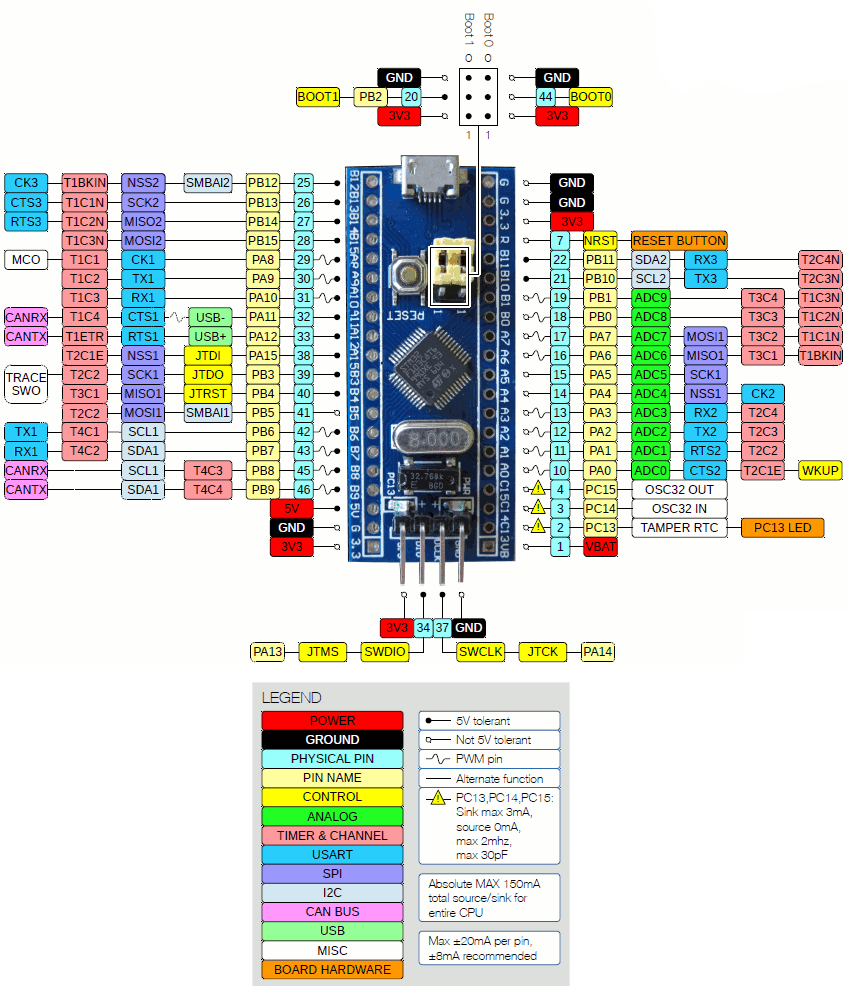
\includegraphics[width=1.0\textwidth]{figures/stm32f1_pinout}
	\caption{Diagrama de pinos do STM32F103C8}
    \label{stm32f103c8_pinout}
\end{figure}

Para carregar o projeto no microcontrolador, tem por padrão o uso do gravador ST-LINK v2.
O ST-link, cujo original (figura \ref{stlinkv2_original}) é fabricado pela ST-Microelectronics \cite{st_link_v2}, 
possui uma versão paralela mais barata
comercializada online (figura \ref{stlinkv2_cheap}), porém a versão paralelo costuma ter fabricantes diversos e 
muitas vezes não descritos na distribuição do produto 
e a relação de pinos pode variar (figura \ref{stlinkv2_cheap_pin_diff}).

\begin{figure}[ht]
	\centering
	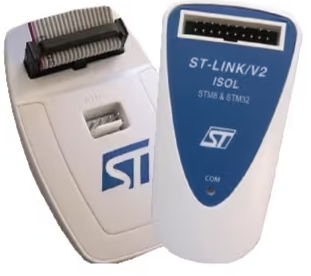
\includegraphics[width=0.5\textwidth]{figures/stlinkv2_original}
	\caption{St-Link V2 original fabricado pela ST-Microelectronics \cite{st_link_v2}}
    \label{stlinkv2_original}
\end{figure}


\begin{figure}[ht]
	\centering
	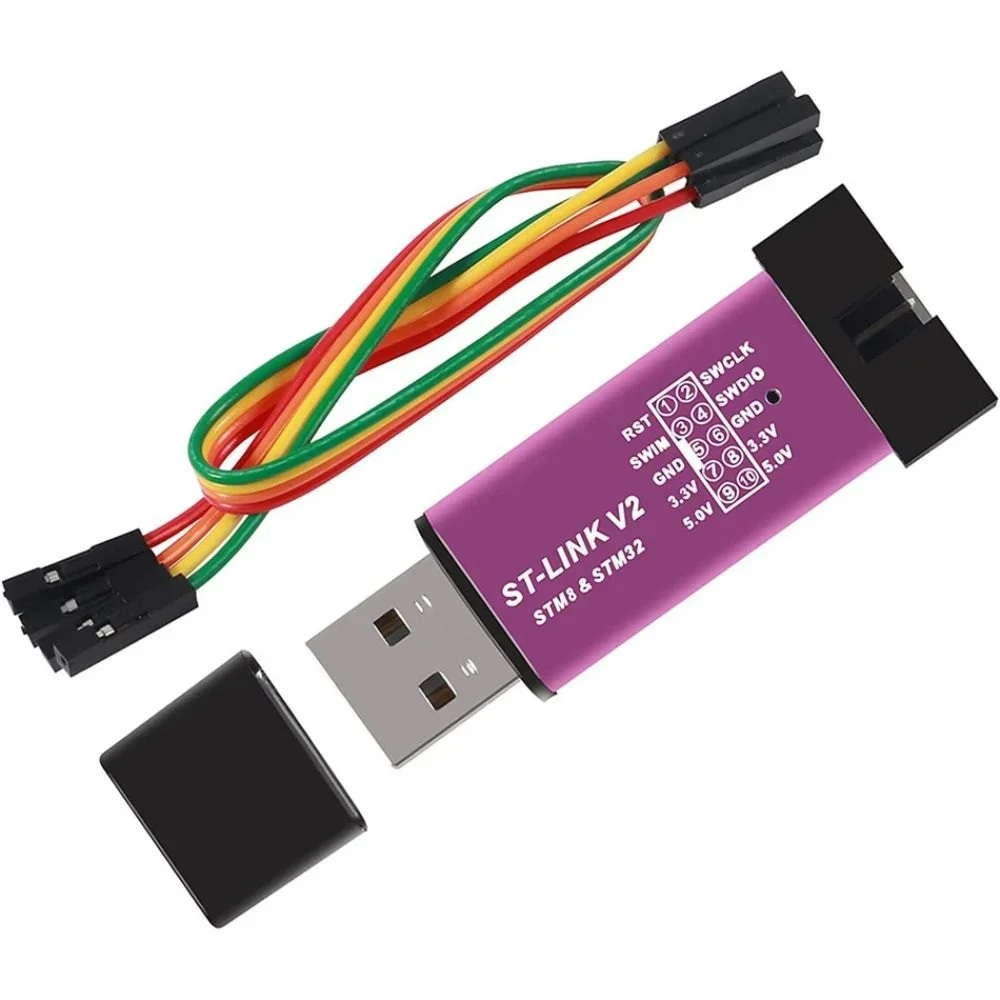
\includegraphics[width=0.5\textwidth]{figures/stlinkv2_cheap}
	\caption{St-Link V2 paralelo de fabricação desconhecida \cite{stlinkv2_cheap_ref}}
    \label{stlinkv2_cheap}
\end{figure}


\begin{figure}[htb]
	\centering
	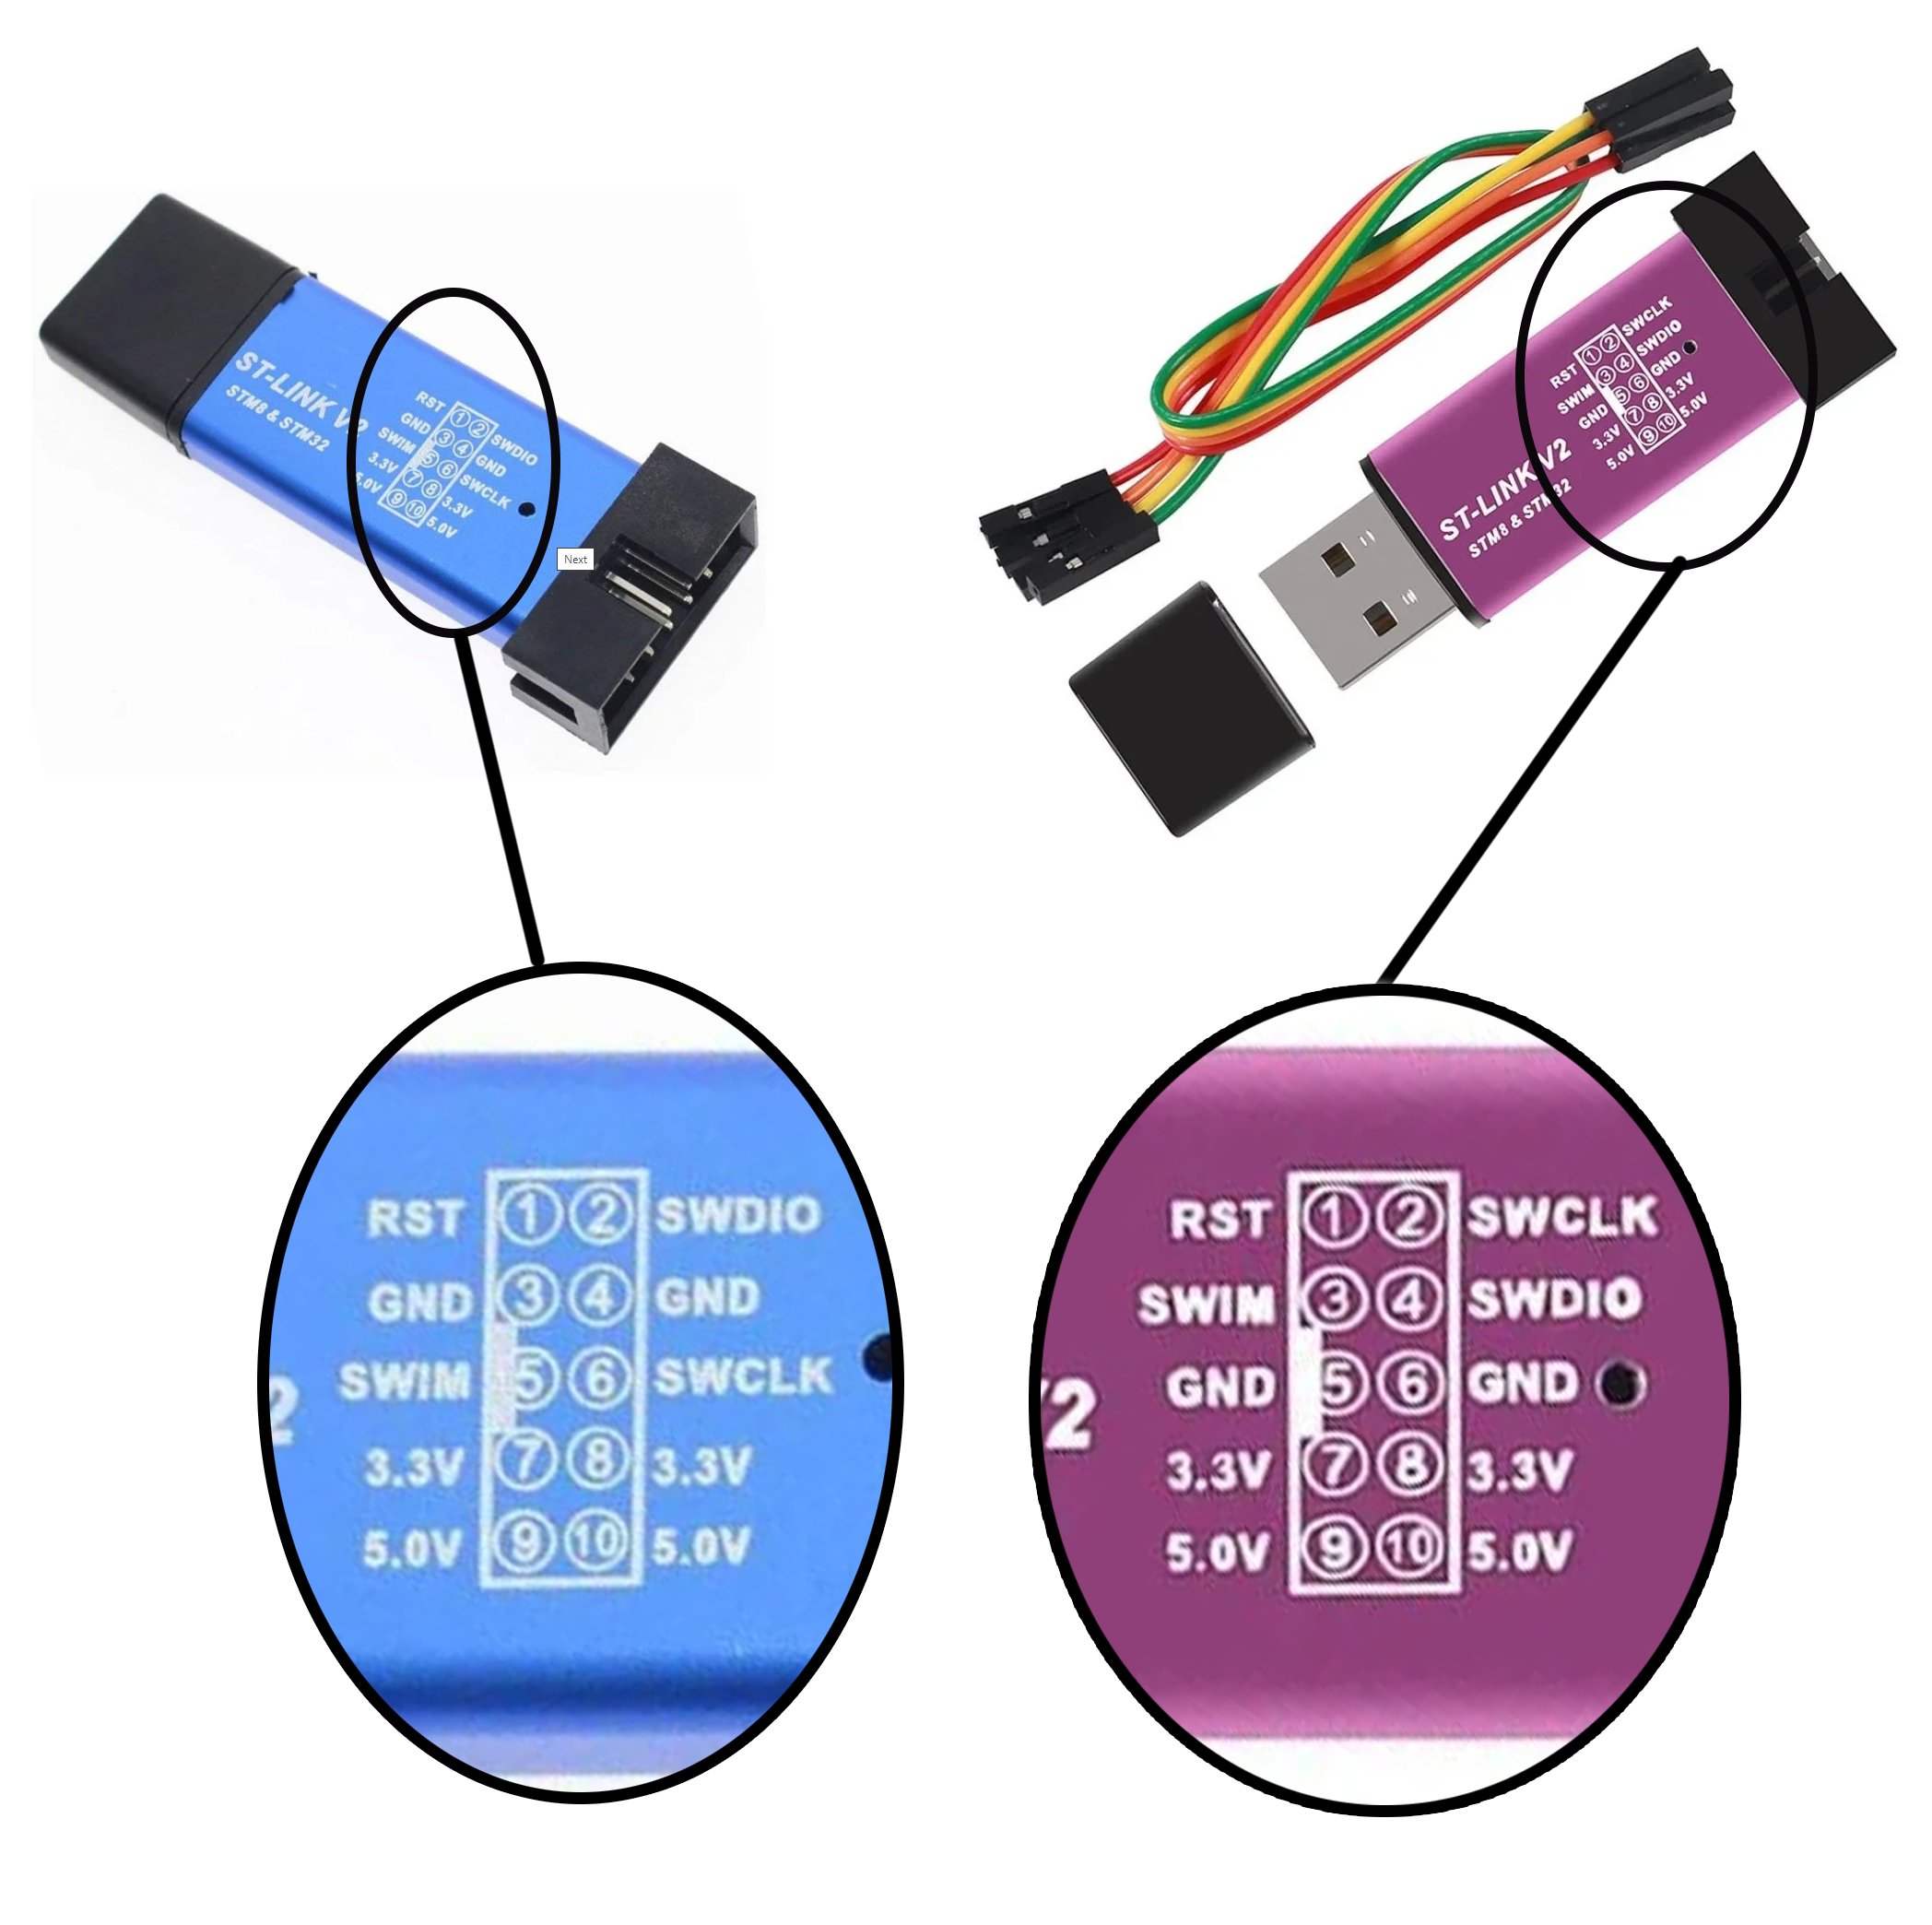
\includegraphics[width=0.5\textwidth]{figures/stlinkv2_cheap_pin_diff}
	\caption{St-Link V2 paralelo e o problema da não padronização de pinos
		(figura obtida ampliando as figuras disponíveis em \cite{stlinkv2_cheap_ref} e \cite{stlinkv2_cheap_pin_diff_ref})
	}
    \label{stlinkv2_cheap_pin_diff}
\end{figure}

A partir daqui todas as menções a "STM32" são referem diretamente a  placa BluePill.


\subsection{ESP32 Devkit v1}

A placa ESP32 Devkit v1, de fabricação da DOIT.am, ela possui o microcontrolador ESP32-WROOM-32E (figura \ref{esp32_pinout}) fabricado pela Espressif Systems
A série ESP32 foi lançada em 2016 \cite{anuncio_esp32}, e possui arquitetura de 32 bits
tem se tornado popular por possuir opções com integração bluetooth e wifi.
O ESP32-WROOM-32E possui um processador dual core ESP32-D0WD-V3 \cite{esp32_wroom_32e_datasheet}, com frequência máxima de 240MHz, wi-fi 2.4Ghz de até 150Mbps e
bluetooth 4.2. Em relação aos periféricos, embora a placa tenha 48 GPIOs, elas estão endereçadas em apenas 25 pinos.
Entre os periféricos existem 15 canais ADC, 2 interfaces UART, 
2 canais DAC, 25 PWM, uma interfade de SPI, I2C e I2S, e 9 interface de toque capacitivo \cite{esp32_reference_2} \cite{esp32_reference}.

\begin{figure}[ht]
	\centering
	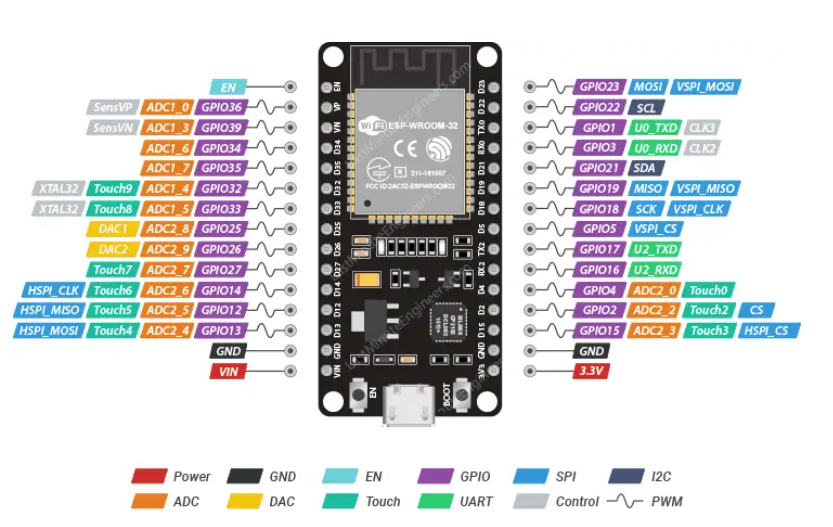
\includegraphics[width=1.0\textwidth]{figures/esp32_pinout}
	\caption{Diagrama de pinos do ESP32 Devkit v1 \cite{esp32_reference}}
	\label{esp32_pinout}
\end{figure}

De acordo com alguns artigos dispoíveis online sobre o ESP32 Devkit v1  \cite{esp32_reference_2} e \cite{esp32_reference},
nem todos os 25 pinos são totalmente livres para usar,
alguns possuem limitações de uso de acordo como periférico em uso. a figura \ref{esp32_pinout_ref}

\begin{figure}[ht]
	\centering
	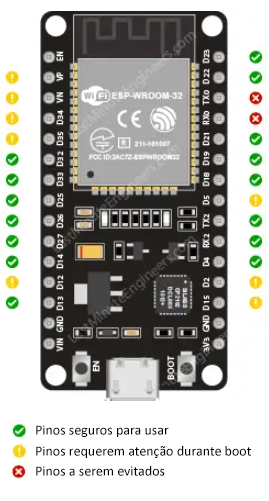
\includegraphics[width=0.35\textwidth]{figures/esp32_pinout_ref}
	\caption{Recomendação de uso dos pinos do ESP32 Devkit v1 \cite{esp32_reference}}
	\label{esp32_pinout_ref}
\end{figure}

Diferente do STM32 o ESP32 Devkit v1 pode ser gravado diretamente via USB.

\subsection{Definição da placa para o projeto}

Aqui explico a integração do stm32 duino,  o problema do stlink com usb ao mesmo tempo
e depois falo sobree as vantagens do esp32.